\section{Where do the electrons flow?}

\begin{enumerate}
    \item Solve for the currents in each of the branches ($i_3, i_4, i_7$)
        shown in the following circuit shown in Figure~\ref{fig:p1vs}.

    \begin{figure}[h!]
    \begin{minipage}[l]{0.75\linewidth}
    \centering
    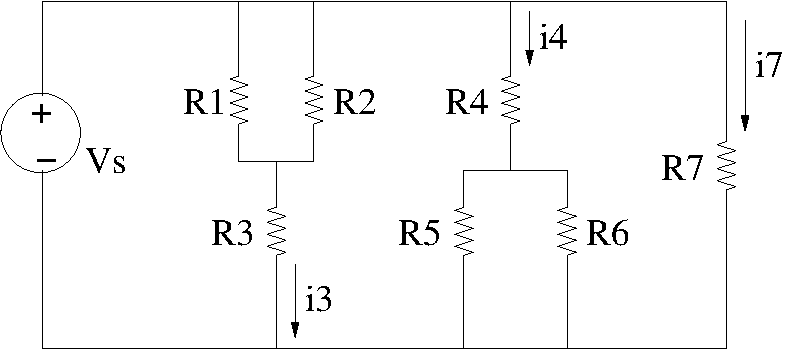
\includegraphics[width=0.75\linewidth]{p1/p1vs}
    \caption{Voltage Source Circuit}
    \label{fig:p1vs}
    \end{minipage}\hfill
    \begin{minipage}[l]{0.25\linewidth}
    \vspace*{-0.25in}
    \begin{tabular}{|l|l|}
    \hline
    Component & Value \\ \hline
    $V_s$ & 9 V \\ \hline
    $R_1$ & 10 $\Omega$ \\ \hline
    $R_2$ & 10 $\Omega$ \\ \hline
    $R_3$ & 5 $\Omega$ \\ \hline
    $R_4$ & 10 $\Omega$ \\ \hline
    $R_5$ & 20 $\Omega$ \\ \hline
    $R_6$ & 20 $\Omega$ \\ \hline
    $R_7$ & 30 $\Omega$ \\ \hline
    \end{tabular}
    \end{minipage}
    \end{figure}

    \item How much power is supplied by the voltage source (magnitude only)?

    \item Solve for the new branch currents ($i_3, i_4, i_7$) when a current
        source is substituted for the voltage source:

    \begin{figure}[h!]
    \begin{minipage}[l]{0.75\linewidth}
    \centering
    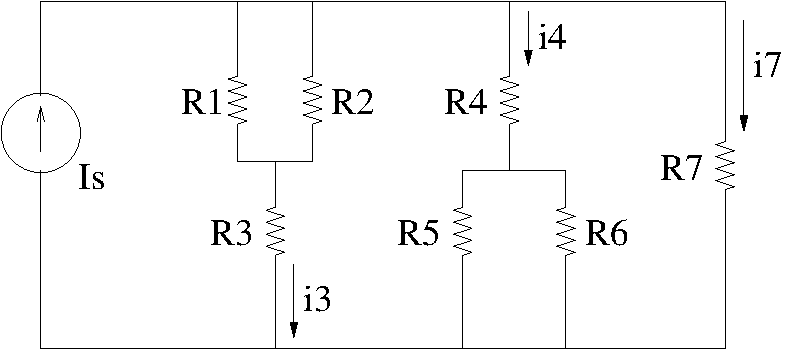
\includegraphics[width=0.75\linewidth]{p1/p1}
    \caption{Current Source Circuit}
    \label{fig:p1}
    \end{minipage}\hfill
    \begin{minipage}[l]{0.25\linewidth}
    \vspace*{-0.25in}
    \begin{tabular}{|l|l|}
    \hline
    Component & Value \\ \hline
    $I_s$ & 11 A \\ \hline
    $R_1$ & 10 $\Omega$ \\ \hline
    $R_2$ & 10 $\Omega$ \\ \hline
    $R_3$ & 5 $\Omega$ \\ \hline
    $R_4$ & 10 $\Omega$ \\ \hline
    $R_5$ & 20 $\Omega$ \\ \hline
    $R_6$ & 20 $\Omega$ \\ \hline
    $R_7$ & 30 $\Omega$ \\ \hline
    \end{tabular}
    \end{minipage}
    \end{figure}

    \item How much power is supplied by the current source (magnitude only)?

\end{enumerate}
